\section{Application: temps d'attente dans les aéroports}
En assurant un \textbf{contrôle pré-embarquement} efficace et efficient, l'\textit{Administration canadienne de la sûreté du transport aérien} (ACSTA) assure la sécurité de tous les passagers et de l'équipage à bord des vols quittant les aéroports canadiens, tout en maintenant un équilibre approprié entre les effectifs du personnel de contrðle et le temps d'attente des passagers. \par Le nombre de postes de contrôle actifs et le nombre de passagers ont une incidence sur les temps d'attente et, par conséquent, les réductions budgétaires ont un impact important sur le système.\newl
De nombreux facteurs influencent le temps d'attente aux points de contrôle dans les aéroports canadiens: l'intensité des horaires des vols, le volume de passagers sur ces vols, le nombre de serveurs et les taux de traitement à un point de contrôle donné, etc. \par L'un des objectifs de l'ACSTA est de faire en sorte que l'expérience du contrôle préembarquement dans les aéroports canadiens soit la plus efficace possible en réduisant au minimum le temps d'attente aux points de contrôle. Dans cette optique, le \textbf{modèle d’impact sur l’attente} (``Wait-Time Impact Model'’ — WTIM) a été conçu afin de réaliser les tâches suivantes: 
\begin{enumerate}[noitemsep]
\item fournir des estimés des taux d'arrivée des passagers ($\lambda$), des taux de traitement ($\mu$) et du nombre de serveurs ($c$) à chaque point de contrôle, en utilisant les données disponibles sur le terrain;
\item calculer le niveau de qualité de service (QdS) $(p_x,x)$ et déterminer quel niveau de service peut être atteint à chaque point de contrôle (c'est-à-dire, le pourcentage $p$ de passagers qui attendront moins de $x$ minutes, pour $x$ fixe) pour un taux d'arrivée donné $\lambda$, taux de traitement $\mu$, nombre de serveurs $c$;
\item obtenir le nombre moyen de serveurs $c^*$ requis pour atteindre un niveau de qualité de service prescrit $(p_x,x)$, compte tenu d'un profil d'arrivée $\lambda^*$;
\item fournir des courbes de niveau de QdS $(p_x(x),x)$ (c'est-à-dire des courbes de distribution cumulative) en fonction de divers taux d'arrivée et du nombre de serveurs actifs pour chaque point de contrôle (où $x$ varie).\end{enumerate}
\begin{figure*}[!t]
\centering
\includegraphics[height=0.35\textheight]{Images/CATSA2_\ldoc.png}\quad 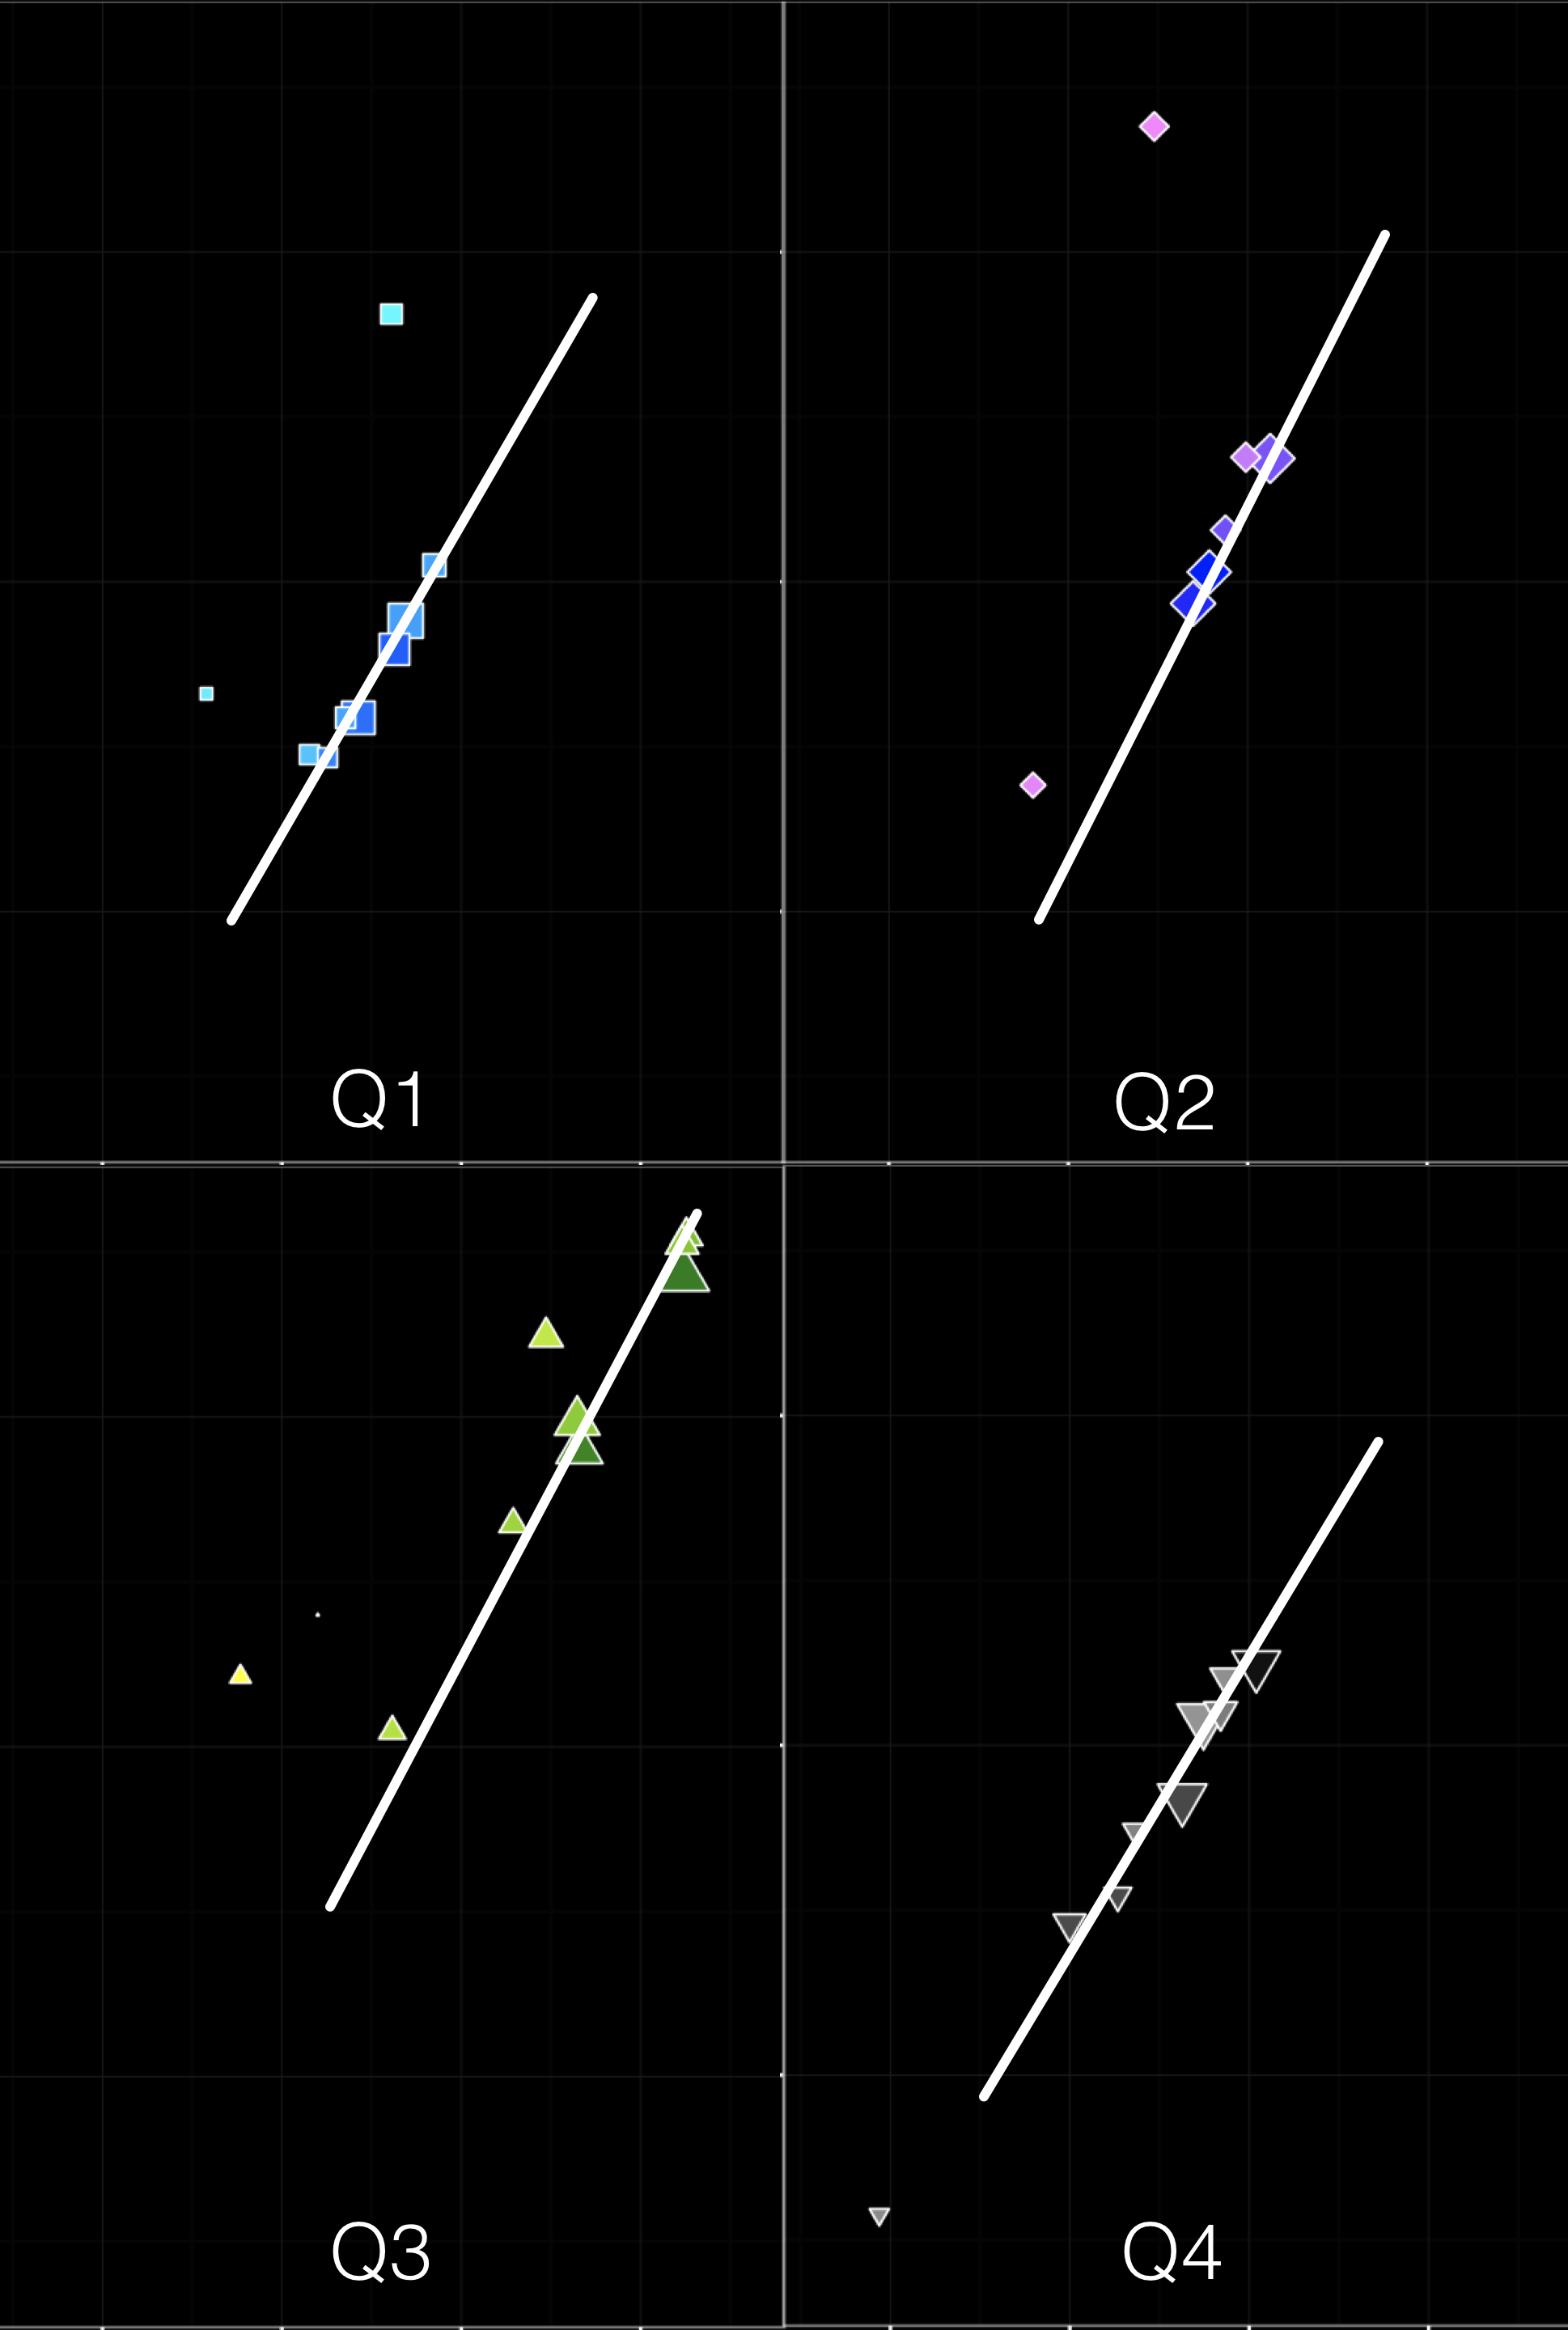
\includegraphics[height=0.35\textheight]{Images/CATSA3.png} \\  \ \\ 
\includegraphics[width=0.60\textwidth]{Images/CATSA4_\ldoc.png}  
\caption{\small En haut: visualisation des paramètres de file d'attente d'un point de contrôle spécifique -- $\lambda$, $\mu$, $\bar{c}$, nombre de passagers et performance (pourcentage de voyageurs attendant moins de 15 minutes pour être contrôlés); la relation entre $\lambda/\bar{c}$ et $\mu/\bar{c}$ est pratiquement linéaire (à gauche), ce qui est plus facile à voir au niveau des trimestres (à droite). En bas: prédiction du nombre moyen de serveurs par rapport au nombre réel de serveurs nécessaires pour maintenir les performances prescrites, avec le nombre de passagers, par trimestre. La ligne de prédiction idéale est ajoutée pour faciliter la comparaison.}\label{fig:checkpoint}\hrule
\end{figure*} 
La structure de la file d'attente permet d'obtenir des informations intéressantes (comme on peut le constater à la  Figure~\ref{fig:checkpoint}). Plus de détails sont disponibles dans la présentation qui accompagne ce rapport.